% chapters/00_cover.tex
% Trang bìa (có đường viền và logo) for HCMUT Master's Thesis
% Theo mẫu biểu mẫu 10
% Author: Nguyễn Tấn Khôi
% Date: 2025-12-14

%% ============================================================================
%% TRANG BÌA (BÌA CHÍNH) - CÓ ĐƯỜNG VIỀN VÀ LOGO
%% ============================================================================

\begin{titlepage}

% Double border around cover page
\begin{tikzpicture}[remember picture,overlay]
  % Outer border (2pt thick)
  \draw[line width=2pt]
    ([xshift=2cm,yshift=-2cm]current page.north west)
    rectangle
    ([xshift=-1cm,yshift=2cm]current page.south east);

  % Inner border (1pt thick, 3mm inside outer)
  \draw[line width=1pt]
    ([xshift=2.3cm,yshift=-2.3cm]current page.north west)
    rectangle
    ([xshift=-1.3cm,yshift=2.3cm]current page.south east);
\end{tikzpicture}

\begin{center}

% Tên trường
{\fontsize{14}{16}\selectfont
ĐẠI HỌC QUỐC GIA TP. HCM\\
\textbf{TRƯỜNG ĐẠI HỌC BÁCH KHOA}\\[0.3cm]
--------------------
}


% Logo
% 
\includegraphics[width=3cm]{images/bk-logo.png}

\vspace{2cm}

% Họ và tên học viên (in đậm)
{\fontsize{15}{16}\selectfont\bfseries
\MakeUppercase{\authorname}\\
}

\vspace{2cm}

% Tên đề tài (in đậm, cỡ lớn hơn)
{\fontsize{16}{19}\selectfont\bfseries
\MakeUppercase{\thesistitleVN}\\
}

\vspace{1.5cm}

\begin{center}
{\fontsize{13}{15}\selectfont
\begin{tabular}{@{}l l@{}}
Chuyên ngành: & \major \\
Mã số:        & \majorcode \\
\end{tabular}
}
\end{center}

\vspace{2cm}

% LUẬN VĂN THẠC SĨ
{\fontsize{21}{24}\selectfont\bfseries
LUẬN VĂN THẠC SĨ\\
}

\vfill

% Địa điểm và thời gian
{\fontsize{13}{15}\selectfont
TP. HỒ CHÍ MINH, tháng 12 năm 2025\\
}

\end{center}
\end{titlepage}
